\subsection{Gantry control and hardware}
\label{sec:gantry}

This subsection describes the motion-control program and the hardware it drives (functional units FU~2.8 and FU~3.1 to FU~3.4; requirement R5). The single-board computer generates the step and direction pulses of both stepper drivers itself on its general-purpose pins, with no microcontroller in between.
The reason is that a move handed to a microcontroller cannot be interrupted without a round trip, whereas in the implemented design the loop that emits every step also reads the end-stop switches, so ``stop at once on any trigger'' is a property of the program; an earlier design with a microcontroller on a serial link was superseded for this reason.
The interpreter (about 800 lines of Python), the calibration and the safety logic were written by the student; the only library used gives access to the pins.

\subsubsection{Components, and why each was chosen}
\label{sec:gan-components}

Table~\ref{tab:gan-bom} lists the electrical and mechanical components and the reason each was selected. Every one was bought rather than designed, so no credit is claimed for the parts themselves; what is claimed is the selection, the interface circuits around them and the control program.
Table~\ref{tab:gan-pins} gives the pin assignment of the control program, and Table~\ref{tab:gan-hw} records, item by item, what the project files evidence --- including the transmission values the program assumes --- together with the information that must still be supplied.

\begin{table}[!htbp]
\centering
\fontsize{8.5}{10.2}\selectfont
\begin{tabularx}{\linewidth}{|>{\raggedright\arraybackslash}p{3.5cm}|>{\raggedright\arraybackslash}p{2.6cm}|>{\raggedright\arraybackslash}X|}
\hline
\textbf{Component} & \textbf{Quantity and rating} & \textbf{Reason for the choice} \\
\hline
Single-board computer, ODROID N2+ & 1 & The proposal requires all processing on an embedded platform. It runs the networks, the server and the motion control on one board, and its 3.3\,V pins are driven directly from the motion program. \\
\hline
Stepper motor, NEMA 17 & 2, 1.68\,A per phase~\cite{stepperds} & A stepper gives open-loop position from a step count~\cite{acarnley2002}, so no encoder is needed for the resolution R5 asks for. The NEMA 17 frame is the standard size for which the belts, pulleys and brackets used here are made. \mustdo{confirm the manufacturer, exact model number and datasheet revision or date of the stepper motors actually fitted, together with the rated phase current, step angle and the torque--speed curve; the bibliography entry carries none of these because the part could not be identified from the project files.} \\
\hline
Stepper driver, A4988 carrier~\cite{a4988ds} & 2 & Takes one STEP and one DIR line per axis, which is the smallest pin count for the job, and chops the coil current so the 1.68\,A winding can be run from the 24\,V rail. Microstepping to 1/16~\cite{acarnley2002,a4988ds} is set by jumpers and multiplies the resolution of Equation~\ref{eq:gan-spm} by sixteen. \mustdo{confirm the manufacturer, exact part number and datasheet revision or date of the driver carriers actually fitted (Allegro A4988 is assumed), since the carrier variant also fixes the sense-resistor value used in Equation~\ref{eq:gan-current}.} \\
\hline
Power supply & 1, 24\,V & A higher rail forces current into the winding inductance faster, which is what allows the step rates of Section~\ref{sec:gan-res}; 24\,V is inside the A4988's 8 to 35\,V input range~\cite{a4988ds}. \\
\hline
Bulk capacitor & 1, 100\,\textmu F & Supplies the switching current of the drivers locally so the rail does not sag at each chop (Equation~\ref{eq:gan-bulk}). \\
\hline
Micro switch & 5 & Four as the end-stops of the two axes, which make the direction-agnostic calibration of Section~\ref{sec:gan-calib} and the emergency stop possible; the fifth reports the state of the pen cam. A mechanical switch was chosen over an optical sensor because it needs no supply of its own and cannot be confused by ambient light. \\
\hline
Pull-down resistor & 4, 10\,k$\Omega$ & Holds each switch input low when the switch is open, so the input is never floating (Equation~\ref{eq:gan-pull}). \\
\hline
Pen-lift motor, N20 gear motor & 1, 150\,rpm & Geared down enough to turn the cam that toggles the pen in one direction. Its speed sets the toggle time, which Section~\ref{sec:gan-pen} shows is the largest single contributor to the predicted writing time. \\
\hline
Switching transistor, BC337-40, with 1\,k$\Omega$ base resistor & 1 & A general-purpose pin cannot supply the pen motor's current, so the pin switches the motor through a transistor instead (Equation~\ref{eq:gan-base} and Figure~\ref{fig:gan-pen-ckt}). \\
\hline
Timing belt and pulleys, GT2 2\,mm pitch, 20 teeth, with idler pulleys & 2 axes & A belt was chosen over a lead screw because the long, light travel of this machine needs speed more than it needs force, and because belt backlash can be kept small by tensioning with the idlers. 2\,mm pitch on 20 teeth gives the 40\,mm per revolution of Equation~\ref{eq:gan-spm}. \\
\hline
Chromed steel rods, linear bearings, 5\,mm to 8\,mm shaft coupler & as required & The rods and bearings carry the carriage so the belt only has to pull it, and the coupler joins the 5\,mm motor shaft to the 8\,mm cross-shaft described in Section~\ref{sec:gan-mech}. \\
\hline
USB camera in a printed housing & 1 & Fixes the camera at a known height above the page and clamps the paper flat, which is what makes the illumination correction of Section~\ref{sec:segmentation} work on a page that would otherwise curl. \\
\hline
\end{tabularx}
\caption{Components of the gantry and the capture rig, with the reason for each choice. All parts were bought; the interface circuits and the control program around them are the student's own work.}
\label{tab:gan-bom}
\end{table}

\mustcomplete{Add to Table~\ref{tab:gan-bom} the exact part numbers and the supplier of the motors,
the driver carrier boards, the power supply and the camera, together with the power supply's current
or VA rating, the camera's model and resolution, and the height at which the housing holds it above
the page. Also state how the 24\,V rail is converted to the voltages the ODROID~N2+ and the pen
motor need, because the board itself is not a 24\,V part and no converter is documented in the
project files.}

The twelve pins of Table~\ref{tab:gan-pins} are all the program needs: two outputs per axis, four switch inputs, and one input and one output for the pen mechanism. They are requested from \texttt{/dev/gpiochip0} in a single call, so a second instance of the program cannot claim the same pins while a job is running.

\begin{table}[!htbp]
\centering
\fontsize{9.5}{11.5}\selectfont
\begin{tabularx}{\linewidth}{|X|c|c|c|c|}
\hline
\textbf{Function} & \textbf{Offset} & \textbf{Header pin} & \textbf{Direction} & \textbf{Initial level} \\
\hline
X motor DIR / STEP & 64 / 68 & 7 / 11 & output & high / low \\
\hline
Y motor DIR / STEP & 81 / 69 & 12 / 13 & output & high / low \\
\hline
X\_MIN / X\_MAX switch & 72 / 65 & 15 / 16 & input & --- \\
\hline
Y\_MIN / Y\_MAX switch & 66 / 67 & 18 / 22 & input & --- \\
\hline
Pen-position switch & 70 & 33 & input & --- \\
\hline
Pen motor drive & 71 & 35 & output & low \\
\hline
\end{tabularx}
\caption{Pin assignment of the gantry driver on \texttt{/dev/gpiochip0}, requested in one call; the header pin numbers are those of the program comments and were not checked against the board pinout.}
\label{tab:gan-pins}
\end{table}

Table~\ref{tab:gan-hw} is the honest statement of how far the hardware description can be taken from the project files alone. Every entry marked in it is outstanding, and the two most serious gaps --- the power supply's rating and whether any level shifter lies between the 3.3\,V pins and the drivers --- bear directly on Section~\ref{sec:gan-supply}.

\begin{table}[!htbp]
\centering
\fontsize{9.5}{11.5}\selectfont
\begin{tabularx}{\linewidth}{|p{2.6cm}|X|}
\hline
\textbf{Item} & \textbf{Evidence, and content to be supplied} \\
\hline
Computer & ODROID N2+ with 3.3\,V pins (Table~\ref{tab:gan-pins}). \\
\hline
Motors, drivers, transmission & Two motors with STEP/DIR driver modules; the program assumes 200 full steps per revolution~\cite{stepperds}, an A4988 at 1/16 microstepping~\cite{a4988ds} and 40\,mm per revolution (2\,mm belt, 20-tooth pulley), and replaces the last by calibration. \mustdo{motor model, holding torque, rated current; driver model, current-limit setting, microstepping jumpers, minimum STEP pulse width; belt or screw type, pulley teeth, guides; whether any level shifter lies between the 3.3\,V pins and the drivers.} \\
\hline
Travel & Measured switch-to-switch distances 204\,mm (X) and 262\,mm (Y). \mustdo{the calibrated steps per millimetre printed for both axes.} \\
\hline
End-stops & Four switches, active-high at 3.3\,V, each with a pull-down of about 10\,k$\Omega$ (Figure~\ref{fig:gan-switch}). \mustdo{switch type and mounting.} \\
\hline
Pen mechanism & One-direction gear motor whose cam toggles the pen every $90^\circ$, with a pen switch (high = up) (Section~\ref{sec:gan-pen}). \mustdo{how the motor is switched (transistor, flyback diode), supply voltage, pen model and holder, lift height.} \\
\hline
Power supply (FU 4) & \mustdo{voltages and current ratings of the motor, computer and pen-motor supplies, grounding scheme, camera supply.} The program comments state that the motors have no flyback diodes and share a ground return, which makes the switch inputs noisy (Section~\ref{sec:gan-stop}). \\
\hline
Camera (FU 1) & Generic USB video-class camera. \mustdo{model, resolution, mounting height, field of view, lamp.} \\
\hline
\end{tabularx}
\caption{Hardware items: evidence in the project files and information still to be supplied.}
\label{tab:gan-hw}
\end{table}

\subsubsection{Mechanical arrangement}
\label{sec:gan-mech}

The machine is a Cartesian gantry of two axes, one motor and one belt each, and the chain is best followed body by body.
The lower axis carries the whole upper axis and is driven by one motor whose shaft is joined, through the 5\,mm to 8\,mm coupler, to an 8\,mm cross-shaft spanning the frame.
That one shaft turns a pulley at each end, so both sides of the moving bridge are driven from the same motor and advance by the same amount; this is what keeps the bridge square to the frame without a second motor and without the electronic synchronisation two motors would need.
The second motor rides on that bridge and drives a single pulley, which moves the carriage along the bridge.
The pen-lift motor and its cam ride on that carriage, so the pen is the last body in the chain and the only mass that has to be moved by the smaller of the two belt loops.
All moving parts run on linear bearings over chromed steel rods, and each belt is tensioned against an idler pulley.

Putting the second motor on the moving bridge is the main mechanical trade-off of the design: it keeps each axis to one motor and one belt, but the lower axis then has to accelerate the upper motor's mass as well as the carriage, which lowers the acceleration that axis can reach before it loses steps.
The alternative, a fixed second motor with a longer belt routed through the bridge, removes that mass but adds idlers and a belt path that changes length as the bridge moves.
The simpler arrangement was chosen because the writing speed turned out to be limited by the search in Section~\ref{sec:synthesis} and by the pen toggle, not by how fast the axes can be accelerated.

The torque each motor must supply follows from the pulley's pitch radius.
For a belt of pitch $p$ on a pulley of $N_t$ teeth the travel per revolution and the pitch radius are given by Equation~\ref{eq:gan-radius},
\begin{equation}
\ell_{\mathrm{rev}}=p\,N_t=2\cdot20=40\ \mathrm{mm},\qquad r=\frac{\ell_{\mathrm{rev}}}{2\pi}=\frac{40}{2\pi}=6.37\ \mathrm{mm},
\label{eq:gan-radius}
\end{equation}
From the pitch radius of Equation~\ref{eq:gan-radius}, the torque needed to accelerate a carriage of mass $m$ at acceleration $a$ against a friction force $F_f$ is
\begin{equation}
T=r\,(m\,a+F_f).
\label{eq:gan-torque}
\end{equation}
Equation~\ref{eq:gan-torque} is the check that decides whether the motors can follow the step rates of Section~\ref{sec:gan-res} without stalling, and it is the calculation this design is missing: neither the carriage masses nor the friction force was measured, and the motors' pull-out torque at the rates used~\cite{acarnley2002,stepperds} was not obtained, so no torque margin can be stated.
This is the reason the program uses no acceleration ramp and why Section~\ref{sec:gan-res} can only warn that abrupt starts may lose steps.

Figure~\ref{fig:gan-photo} is the place where the photographs of the built machine belong. They are design evidence rather than decoration, because the mechanical chain above and the component choices of Table~\ref{tab:gan-bom} can only be checked against the assembled gantry, and the folder intended for them in the project files is empty.

\begin{figure}[!htbp]
\centering
\figplaceholder{2.4cm}{Photographs of the assembled gantry (axes, end-stops, pen holder with toggle motor, paper holder) and of the scanning rig with camera; CAD renderings and a wiring diagram with component values. To be supplied by the student.}
\caption{Photographs of the gantry and the scanning rig (placeholder).}
\label{fig:gan-photo}
\end{figure}

\mustdo{Weigh the two carriages and measure or estimate the friction force, then evaluate
Equation~\ref{eq:gan-torque} at the 400\,mm/s$^2$ of Equation~\ref{eq:gc-trap} and compare the result
with the pull-out torque of the motors at 1200 and 3200 steps per second taken from their torque-speed
curve. State the resulting margin. Also insert the CAD drawings of the gantry and the camera housing
and the photographs of the built machine (Figure~\ref{fig:gan-photo}); the folder intended for them in
the project files is empty, so nothing could be reproduced here.}

\subsubsection{Stepper driver and the coil-current setting}
\label{sec:gan-driver}

Each driver is wired as in Figure~\ref{fig:gan-wiring}: the 24\,V rail and the bulk capacitor to the motor supply pins, the four coil wires to the two output pairs, and STEP and DIR to two pins of the single-board computer. The A4988 chops the coil current, and the current it regulates to is set by a trimmer reference voltage together with the two current-sense resistors of the carrier board, Equation~\ref{eq:gan-current}, which is the relation given in the driver's datasheet~\cite{a4988ds},
\begin{equation}
I_{\mathrm{coil}}=\frac{V_{\mathrm{ref}}}{8\,R_S}\qquad\Longrightarrow\qquad V_{\mathrm{ref}}=8\,R_S\,I_{\mathrm{coil}}.
\label{eq:gan-current}
\end{equation}
For the 1.68\,A rating of these motors and the 0.1\,$\Omega$ sense resistors most commonly fitted to these carriers, Equation~\ref{eq:gan-current} asks for $V_{\mathrm{ref}}=8\cdot0.1\cdot1.68=1.34$\,V.
The motors should not in fact be run at their full rating on this driver.
The current the A4988 regulates to flows through the driver's output transistors, and the heat it produces, $P\approx2I_{\mathrm{coil}}^2R_{DS(\mathrm{on})}$ per driver, has only the small carrier board to leave through, which is why a carrier without a heatsink or forced air is usually held to about 1\,A per phase rather than to the 1.68\,A of Equation~\ref{eq:gan-current}.
Accordingly $V_{\mathrm{ref}}$ is set to about $0.8$\,V on a 0.1\,$\Omega$ board, which trades holding torque for a driver that does not go into thermal shutdown part way through a page; losing a step to an overheating driver costs more accuracy than the lower holding torque does.

\mustdo{Confirm three things about Equation~\ref{eq:gan-current}, because the setting cannot be
read back from the program. First, the sense-resistor value actually fitted to these carrier boards
(0.05, 0.068 and 0.1\,$\Omega$ are all sold) --- read it off the board or measure it. Second, the
voltage the trimmer is actually set to, measured at the reference pin with a multimeter, and the coil
current that Equation~\ref{eq:gan-current} then gives. Third, whether the drivers have heatsinks or a
fan, and whether a thermal shutdown was ever observed during a long job. State the resulting coil
current as a fraction of the 1.68\,A rating.}

\subsubsection{Switch inputs}
\label{sec:gan-switch}

Figure~\ref{fig:gan-switch-ckt} shows one switch input; all five are identical. The switch connects the pin to 3.3\,V when it closes, and a 10\,k$\Omega$ resistor to ground holds the pin low when it is open, so the input is defined at all times.
The current drawn while a switch is closed and the worst case with all four end-stops closed follow from Ohm's law, Equation~\ref{eq:gan-pull},
\begin{equation}
I_{\mathrm{pull}}=\frac{V_{DD}}{R}=\frac{3.3}{10\,000}=0.33\ \mathrm{mA},\qquad 4I_{\mathrm{pull}}=1.3\ \mathrm{mA},
\label{eq:gan-pull}
\end{equation}
which is negligible against anything else on the board.
The choice of 10\,k$\Omega$ is bounded from both sides.
Making the pull-down resistor of Equation~\ref{eq:gan-pull} much smaller than 10\,k$\Omega$ wastes current for no benefit; making it much larger lets the pin's own leakage current $I_{\mathrm{leak}}$ lift the open-switch voltage, and to keep that below the input's low threshold $V_{IL}$ the resistor must satisfy $R\le V_{IL}/I_{\mathrm{leak}}$, both quantities being properties of the single-board computer's pins~\cite{odroidn2ds} \mustdo{confirm the exact ODROID-N2+ board revision and the document (hardware technical reference or datasheet) and its date from which $V_{IL}$ and the input leakage current are taken; the bibliography entry carries no revision or date because the board variant could not be confirmed.}.
The resistor also forms a low-pass filter with the pin and cable capacitance, with time constant $\tau_{RC}=R\,(C_{\mathrm{in}}+C_{\mathrm{cable}})$; for 10\,k$\Omega$ and any plausible stray capacitance of tens to hundreds of picofarads this is a few microseconds, which is more than three orders of magnitude below the 6\,ms between the repeated reads of Section~\ref{sec:gan-stop}, so the debounce is entirely a property of the program and not of this circuit.
Figure~\ref{fig:gan-switch} draws the same input as it is documented in the program comments, with the 0.33\,mA of Equation~\ref{eq:gan-pull} marked on it; the origin of the 3.3\,V at the switch is inferred from those comments rather than read off the board, which is why the figure carries a marker of its own.

\begin{figure}[!htbp]
\centering
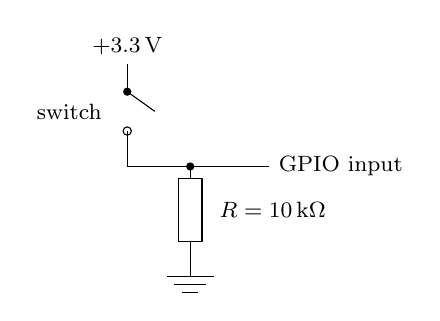
\begin{tikzpicture}[x=1cm,y=1cm,font=\footnotesize]
\draw (0,1.9) node[above] {$+3.3$\,V} -- (0,1.55);
\fill (0,1.55) circle (1.5pt); \draw (0,1.55) -- (0.35,1.3); \draw (0,1.05) circle (1.5pt); \draw (0,1.05) -- (0,0.6);
\node[anchor=east] at (-0.2,1.3) {switch};
\draw (0,0.6) -- (1.8,0.6) node[right] {GPIO input};
\fill (0.8,0.6) circle (1.5pt);
\draw (0.8,0.6) -- (0.8,0.45); \draw[fill=white] (0.65,0.45) rectangle (0.95,-0.35); \draw (0.8,-0.35) -- (0.8,-0.8);
\node[anchor=west] at (1.05,0.05) {$R=10$\,k$\Omega$};
\draw (0.5,-0.8) -- (1.1,-0.8); \draw (0.6,-0.9) -- (1.0,-0.9); \draw (0.7,-1.0) -- (0.9,-1.0);
\end{tikzpicture}
\caption{Switch input circuit as documented in the program comments; the closing current is $3.3\,\mathrm{V}/10\,\mathrm{k}\Omega=0.33$\,mA. The origin of the 3.3\,V (header pin) is inferred and \mustdo{confirm this item}.}
\label{fig:gan-switch}
\end{figure}

The electrical weakness of this arrangement is the return path rather than the resistor.
The motors have no clamp diodes and share a ground return with the switch wiring, so each time a coil is switched its current has to find a path back through that shared conductor: a current $I$ returning through a ground conductor of resistance $R_{gnd}$ raises the local ground by $I\,R_{gnd}$, and the switch inputs are referred to that same ground, so the apparent switch voltage is offset by the same amount.
This is the mechanism behind the behaviour recorded in Section~\ref{sec:gan-stop}, where an input was found to read high for several milliseconds after a motor switched, and it is why a single re-read was not enough and three reads 6\,ms apart were needed.
The correct fix is electrical, not a longer debounce: a clamp diode across each motor, and a switch return brought back to a single ground point separately from the motor current.

\mustdo{For Equation~\ref{eq:gan-pull}, take $V_{IL}$ and the input leakage current from the
ODROID~N2+ documentation~\cite{odroidn2ds} and state the resulting upper bound on the pull-down resistor, so the choice
of 10\,k$\Omega$ is bounded by numbers rather than by argument. Confirm also that each switch is wired
to 3.3\,V and not to 5\,V, since the program reads the inputs as active-high at 3.3\,V.}

\subsubsection{Pen-lift motor and its switching stage}
\label{sec:gan-penckt}

A general-purpose pin can source only a few milliamperes, far below what even a small geared motor draws, so the pen motor is switched by a transistor on the low side as in Figure~\ref{fig:gan-pen-ckt}, the pin driving the base through a 1\,k$\Omega$ resistor. With the pin at 3.3\,V and the base-emitter drop of a saturated small-signal transistor taken as 0.7\,V~\cite{bc337ds} \mustdo{confirm the manufacturer (onsemi and Nexperia both supply this part), the exact part number and the datasheet revision or date of the transistor actually fitted, and check the gain group, $V_{BE(\mathrm{sat})}$, $V_{CE(\mathrm{sat})}$ and TO-92 power dissipation used below against that document; the bibliography entry carries no revision because the variant could not be identified.}, the base current is given by Equation~\ref{eq:gan-base},
\begin{equation}
I_B=\frac{V_{\mathrm{pin}}-V_{BE(\mathrm{sat})}}{R_B}=\frac{3.3-0.7}{1000}=2.6\ \mathrm{mA}.
\label{eq:gan-base}
\end{equation}
The BC337-40 belongs to the $-40$ gain group, whose minimum current gain is 250~\cite{bc337ds}, and to hold it in saturation rather than use it as an amplifier the base must be driven harder than the collector current strictly requires, by an overdrive factor $k_{od}$ of three to five, so the collector current the stage can switch is given by Equation~\ref{eq:gan-ic},
\begin{equation}
I_{C(\max)}=\frac{h_{FE(\min)}\,I_B}{k_{od}}=\frac{250\cdot2.6\ \mathrm{mA}}{k_{od}}=\frac{650\ \mathrm{mA}}{k_{od}},
\label{eq:gan-ic}
\end{equation}
which is 217\,mA at $k_{od}=3$ and 130\,mA at $k_{od}=5$.
The stage is therefore comfortable for a motor drawing up to about 200\,mA and would leave saturation, and begin to dissipate real power, somewhere above that.
The dissipation in the transistor while saturated is $P=V_{CE(\mathrm{sat})}I_C$, which at 200\,mA and a saturation voltage of about 0.7\,V is 0.14\,W, well inside what the TO-92 package can lose without a heatsink~\cite{bc337ds}.

Two things about this stage are not right, and both are stated here rather than in the discussion because they are design faults and not merely untested items.
First, there is no clamp diode across the motor: when the transistor turns off, the energy $\tfrac12LI^2$ stored in the motor's inductance has nowhere to go and appears as a reverse voltage that both stresses the transistor and injects the noise that Section~\ref{sec:gan-switch} describes. A diode across the motor, cathode to the supply, rated for at least the motor current and twice the motor supply voltage, is the standard remedy and was omitted.
Second, there is no base pull-down: the base resistor leaves the base floating while the pin is in its power-up input state, so a pull-down from base to emitter should be fitted to guarantee the motor is off before the program claims the pin.

\mustdo{Measure the pen motor's free-running current and its stall current, then check them
against Equation~\ref{eq:gan-ic}: if the stall current is above about 200\,mA the stage is not hard
saturated and the base resistor should be reduced. State the voltage the pen motor is actually run
from. Confirm whether a clamp diode and a base pull-down were in fact fitted, since neither appears in
the project files; if they were not, this subsection is correct as written and the omission belongs in
Section~\ref{sec:discussion}.}

\subsubsection{Supply and decoupling}
\label{sec:gan-supply}

The 24\,V rail feeds both drivers, and a 100\,\textmu F capacitor is fitted across it close to them to supply the switching current locally, because the chopper in each driver draws current in bursts that the supply leads, which have inductance of their own, cannot follow.
For a current step $I$ lasting $\Delta t$ the rail sags by the amount of Equation~\ref{eq:gan-bulk},
\begin{equation}
\Delta V=\frac{I\,\Delta t}{C},
\label{eq:gan-bulk}
\end{equation}
so a 1.68\,A step lasting 10\,\textmu s drawn from 100\,\textmu F costs $1.68\cdot10\times10^{-6}/100\times10^{-6}=0.17$\,V, which is small against 24\,V and comfortably clear of the driver's undervoltage threshold.
Two gaps remain.
The 100\,\textmu F is shared between the two drivers, whereas the usual recommendation is a bulk capacitor of this order at each driver; and no small ceramic capacitor on the logic supply of either driver is documented, which is the part that suppresses the fast edges rather than the bulk current.
The total supply current also has not been budgeted: it is the sum of two motors at two phases each, the pen motor, the single-board computer and the camera, and without the supply's rating the margin is unknown.

\mustdo{Give the power supply's voltage and current rating and complete the power budget: two
motors at two phases each at the coil current set in Section~\ref{sec:gan-driver}, plus the pen motor,
the ODROID~N2+ and the camera. State the margin that remains. Confirm whether each driver has its own
bulk capacitor and whether a ceramic capacitor is fitted on either driver's logic supply.}

A separate check belongs here because it bears on the only hardware fault in this report.
The driver's STEP, DIR and enable inputs are driven straight from 3.3\,V pins, with no level shifting.
Whether that is correct depends on the voltage the driver needs to see as a logic high, $V_{IH}$, which the driver's datasheet specifies relative to the driver's own logic supply~\cite{a4988ds}: the design is sound if $3.3\,\mathrm{V}>V_{IH}$ with margin, and marginal if it is not.
During commissioning the X axis drove to its first end-stop but the direction pin was not observed to change level on reversal, and that fault was not resolved (Section~\ref{sec:results}).
A level incompatibility is one candidate explanation, but a wiring or configuration fault, a damaged pin and a program fault are equally consistent with what was seen, and no measurement was taken that would separate them.
No cause is claimed here.

\mustcomplete{Resolve the X-axis direction fault, which currently blocks requirement R5 entirely.
Take $V_{IH}$ for the driver's logic inputs from its datasheet and compare it with 3.3\,V to settle
whether level shifting is needed. Then put a meter or a scope on the DIR pin at the pin and again at
the driver, command a reversal, and record whether the level changes at each point. That single
measurement separates a program fault from a wiring fault from a level-compatibility fault, and
nothing further can be said about R5 until it is done.}

\begin{figure}[!htbp]
\centering
\scalebox{0.88}{%
\begin{tikzpicture}[x=1cm,y=1cm,font=\scriptsize,>=latex]
\tikzset{
  blk/.style={draw,thick,rounded corners=2pt,align=center,minimum height=9mm,inner sep=3pt,fill=gray!8},
  mot/.style={draw,thick,circle,minimum size=9mm,fill=white},
  wire/.style={draw,thick},
  pwr/.style={draw,thick,-{Latex[length=2mm]}},
  sig/.style={draw,semithick,-{Latex[length=1.8mm]},dashed}
}
\node[blk,text width=1.9cm] (psu) at (0,0) {24\,V\\supply};
\node[blk,text width=2.1cm] (conv) at (0,-2.4) {24\,V to board\\and pen-motor\\rails};
\node[blk,text width=2.2cm] (sbc) at (0,-4.6) {ODROID N2+\\3.3\,V pins};
\node[blk,text width=2.0cm] (dx) at (4.5,0.7) {A4988\\X axis};
\node[blk,text width=2.0cm] (dy) at (4.5,-1.1) {A4988\\Y axis};
\node[mot] (mx) at (7.8,0.7) {M$_X$};
\node[mot] (my) at (7.8,-1.1) {M$_Y$};
\node[blk,text width=2.2cm] (pen) at (4.5,-3.3) {BC337-40\\1\,k$\Omega$ base};
\node[mot] (pm) at (7.8,-3.3) {M$_P$};
\node[blk,text width=2.4cm] (sw) at (4.5,-5.4) {5 micro switches\\10\,k$\Omega$ pull-downs};
\node[blk,text width=1.9cm] (cam) at (0,-6.3) {USB camera};
% bulk capacitor: shunts the 24 V rail to ground
\draw[wire] (1.55,0) -- (1.55,-0.40);
\draw[wire] (1.27,-0.40) -- (1.83,-0.40);
\draw[wire] (1.27,-0.61) -- (1.83,-0.61);
\draw[wire] (1.55,-0.61) -- (1.55,-0.87);
\draw[wire] (1.25,-0.87) -- (1.85,-0.87);
\draw[wire] (1.36,-0.99) -- (1.74,-0.99);
\draw[wire] (1.48,-1.11) -- (1.62,-1.11);
\node[right,inner sep=3pt] at (2.05,-0.51) {100\,\textmu F};
\fill (1.55,0) circle (0.045);
% power routing
\draw[pwr] (psu.east) -- (3.1,0) |- (dx.west);
\draw[pwr] (3.1,0) |- (dy.west);
\draw[pwr] (psu.south) -- (conv.north);
\draw[pwr] (conv.south) -- (sbc.north);
\draw[pwr] (conv.east) -| (3.2,-3.3) -- (pen.west);
\draw[pwr] (dx.east) -- (mx.west);
\draw[pwr] (dy.east) -- (my.west);
\draw[pwr] (pen.east) -- (pm.west);
% signals
\draw[sig] (sbc.east) -- (2.3,-4.6) |- (dx.south west);
\draw[sig] (2.3,-4.6) |- (dy.south west);
\draw[sig] (2.3,-4.6) |- (pen.north west);
\draw[sig] (sw.west) -- (2.7,-5.4) -| (sbc.south);
\draw[sig] (cam.east) -- (1.6,-6.3) -- (1.6,-5.0) -| (sbc.east);
\node[anchor=west] at (6.45,-4.75) {\textbf{Key}};
\draw[pwr] (6.45,-5.20) -- (6.95,-5.20); \node[right,inner sep=3pt] at (6.95,-5.20) {power};
\draw[sig] (6.45,-5.60) -- (6.95,-5.60); \node[right,inner sep=3pt] at (6.95,-5.60) {signal};
\end{tikzpicture}}
\caption{Wiring of the electronics. The 24\,V rail feeds both drivers and is decoupled by the 100\,\textmu F capacitor of Equation~\ref{eq:gan-bulk}; the board drives STEP and DIR of each driver and the pen-motor transistor's base, and reads the five switches. The conversion from 24\,V to the voltages the board and the pen motor need is not documented in the project files.}
\label{fig:gan-wiring}
\end{figure}

\begin{figure}[!htbp]
\centering
\scalebox{0.88}{%
\begin{tikzpicture}[x=1cm,y=1cm,font=\scriptsize,>=latex]
%% ---------------- (a) switch input ----------------
\begin{scope}
\draw[thick] (-0.7,2.4) -- (1.5,2.4);
\node[right,inner sep=2pt] at (1.5,2.4) {3.3\,V};
\draw[thick] (0,2.4) -- (0,1.88);
\fill (0,1.88) circle (0.05);
\draw[thick] (0.03,1.85) -- (0.62,1.38);
\fill (0,1.16) circle (0.05);
\draw[thick] (0,1.16) -- (0,0.80);
\node[right,align=left] at (0.68,1.62) {micro\\switch};
\fill (0,0.80) circle (0.05);
\draw[thick] (0,0.80) -- (1.45,0.80);
\draw[thick,-{Latex[length=2mm]}] (1.45,0.80) -- (2.05,0.80);
\node[right,align=left,inner sep=2pt] at (2.05,0.80) {to pin\\(active high)};
\draw[thick] (0,0.80) -- (0,0.44);
\draw[thick,fill=white] (-0.17,0.44) rectangle (0.17,-0.16);
\node[left,inner sep=4pt] at (-0.19,0.14) {$10\,\mathrm{k}\Omega$};
\draw[thick] (0,-0.16) -- (0,-0.54);
\draw[thick] (-0.30,-0.54) -- (0.30,-0.54);
\draw[thick] (-0.18,-0.66) -- (0.18,-0.66);
\draw[thick] (-0.07,-0.78) -- (0.07,-0.78);
\node[below,inner sep=3pt] at (0,-0.81) {GND};
\node[font=\footnotesize] at (0.7,-1.42) {(a) one switch input, five identical};
\end{scope}
%% ---------------- (b) pen-motor switching stage ----------------
\begin{scope}[xshift=7.6cm]
\draw[thick] (-1.75,2.6) -- (1.15,2.6);
\node[right,inner sep=2pt] at (1.15,2.6) {$V_{\mathrm{motor}}$};
% motor
\draw[thick] (0,2.6) -- (0,2.18);
\node[draw,thick,circle,minimum size=9mm,fill=white] at (0,1.73) {M$_P$};
\draw[thick] (0,1.28) -- (0,0.88);
\node[right,align=left,inner sep=3pt] at (0.48,1.73) {N20 gear motor,\\pen cam};
% clamp diode, drawn dashed because it is NOT fitted
\draw[red,dashed,thick] (-1.15,2.6) -- (-1.15,2.16);
\draw[red,dashed,thick,fill=red!8] (-1.37,2.16) -- (-0.93,2.16) -- (-1.15,1.80) -- cycle;
\draw[red,dashed,thick] (-1.37,1.80) -- (-0.93,1.80);
\draw[red,dashed,thick] (-1.15,1.80) -- (-1.15,1.40) -- (0,1.40);
\node[left,align=right,red,inner sep=3pt] at (-1.40,2.02) {clamp diode\\\textbf{NOT fitted}};
% NPN transistor
\draw[thick] (0,0.88) -- (0,0.74);
\draw[thick] (-0.28,0.74) -- (-0.28,0.02);
\draw[thick] (-0.28,0.62) -- (0,0.86);
\draw[thick] (-0.28,0.14) -- (0,-0.10);
\draw[thick,-{Latex[length=1.7mm]}] (-0.15,0.03) -- (0,-0.10);
\draw[thick] (0,-0.10) -- (0,-0.50);
\node[right,inner sep=3pt] at (0.10,0.38) {BC337-40};
% base drive, arrow pointing INTO the base resistor
\draw[thick] (-0.28,0.38) -- (-0.72,0.38);
\draw[thick,fill=white] (-1.12,0.20) rectangle (-0.72,0.56);
\node[above,inner sep=2pt] at (-0.92,0.57) {$R_B=1\,\mathrm{k}\Omega$};
\draw[thick,-{Latex[length=2mm]}] (-1.80,0.38) -- (-1.12,0.38);
\node[left,align=right,inner sep=2pt] at (-1.80,0.38) {from pin\\3.3\,V};
% ground
\draw[thick] (-0.30,-0.50) -- (0.30,-0.50);
\draw[thick] (-0.18,-0.62) -- (0.18,-0.62);
\draw[thick] (-0.07,-0.74) -- (0.07,-0.74);
\node[below,inner sep=3pt] at (0,-0.77) {GND};
\node[font=\footnotesize] at (-0.4,-1.42) {(b) pen-motor switching stage};
\end{scope}
\end{tikzpicture}}
\caption{The two interface circuits designed around the bought parts. In (a) the 10\,k$\Omega$ resistor holds the pin at ground until the switch closes, drawing the 0.33\,mA of Equation~\ref{eq:gan-pull}; in (b) the pin drives the base through 1\,k$\Omega$, giving the 2.6\,mA of Equation~\ref{eq:gan-base} and the collector current of Equation~\ref{eq:gan-ic}. The clamp diode shown dashed is the standard protection against the motor's inductive turn-off; it is not fitted in the built circuit, and its absence is the source of the switch-input disturbance of Section~\ref{sec:gan-switch}.}
\label{fig:gan-switch-ckt}
\label{fig:gan-pen-ckt}
\end{figure}

\subsubsection{Step generation, resolution and speed}
\label{sec:gan-res}

A driver advances the motor one microstep per pulse at STEP, in the direction given by DIR.
With 200 full steps~\cite{stepperds}, 16 microsteps per step~\cite{a4988ds} and $\ell_{\mathrm{rev}}=40$\,mm per revolution (assumed values), Equation~\ref{eq:gan-spm} gives the step resolution,
\begin{equation}
\kappa=\frac{200\cdot16}{\ell_{\mathrm{rev}}}=\frac{3200}{40}=80\ \mathrm{steps/mm},\qquad\Delta=\frac1\kappa=12.5\ \mu\mathrm{m},
\label{eq:gan-spm}
\end{equation}
and after calibration $\kappa$ is replaced by the measured value of each axis.
Targets are converted to \emph{absolute} integer step counts, $n_{\mathrm{target}}=\mathrm{round}\bigl((x+5)\kappa\bigr)$ with the 5\,mm edge offset of Section~\ref{sec:gan-calib} and the calibrated resolution $\kappa$ of Equation~\ref{eq:gan-cal}, and the step difference is taken against the tracked integer position, so rounding errors do not accumulate.
The quantisation error is at most $\Delta/2=6.25\ \mu$m per axis and $\sqrt2\,\Delta/2=8.8\ \mu$m combined, 57 times finer than the 0.5\,mm of R5.
This is only the \emph{digital} resolution: the accuracy of a mark is set by belt stretch, backlash, missed steps (open loop, no encoders), switch repeatability and pen compliance, none of which was measured.
\mustdo{measure the positional error for R5 (the same word drawn twice and overlaid) and the return-to-zero repeatability.}

For a move of length $d$ at feed $v_f$ (mm/s) with $N_{\mathrm{maj}}=\max(|n_x|,|n_y|,1)$ steps on the major axis the delay of every pulse is given by Equation~\ref{eq:gan-tau},
\begin{equation}
\tau=\max\Bigl(\frac{d/v_f}{N_{\mathrm{maj}}},\ 2\,\mu\mathrm s\Bigr),\qquad v_f=\max(F/60,\,0.1),
\label{eq:gan-tau}
\end{equation}
with $F$ the feed in mm/min.
For an axis-parallel move, 900\,mm/min gives $\tau=1/(15\cdot80)=833\ \mu$s (1200 steps/s) and 2400\,mm/min gives 312.5\,\textmu s (3200 steps/s, 60\,rpm), while homing and retracting run at 625 steps/s or $7.8$\,mm/s. The real rate is limited by the program (four switch readings and two pin writes per step) and the sleep granularity, not by the 2\,\textmu s floor; the maximum reliable rate and the stall speed were not measured.
\mustdo{measure the highest feed without lost steps.}
Since \emph{every} pulse of both axes sleeps for $\tau$, a segment takes $(n_{\mathrm{maj}}+n_{\mathrm{min}})\tau$ and the effective feed is given by Equation~\ref{eq:gan-eff},
\begin{equation}
v_{\mathrm{eff}}=v_f\,\frac{n_{\mathrm{maj}}}{n_{\mathrm{maj}}+n_{\mathrm{min}}}\in\Bigl[\frac{v_f}{2},v_f\Bigr],
\label{eq:gan-eff}
\end{equation}
$v_f$ for an axis-parallel move and $v_f/2$ at $45^\circ$; for uniformly distributed directions the mean factor is $\frac4\pi\int_0^{\pi/4}\frac{\mathrm d\vartheta}{1+\tan\vartheta}=\frac12+\frac{\ln2}{\pi}=0.72$.
The interpreter executes \emph{no acceleration ramps}: the constant speed of Equation~\ref{eq:gan-tau} is used, and the acceleration of Equation~\ref{eq:gc-trap} appears only in the generator's estimate; abrupt starts at 1200 to 3200 steps/s with an unknown motor and load may lose steps, which is exactly the failure that controlled acceleration within the torque--speed envelope is meant to prevent in an open-loop drive~\cite{acarnley2002}.
\label{sec:gan-timing}
A model of the interpreter for the test word of Section~\ref{sec:gcode} (modal feed, Equation~\ref{eq:gan-eff}, first travel at 2400\,mm/min) gives 6.8\,s drawing, 10.8\,s travel and 9.1\,s dwell, 26.7\,s in total (2.4\,s per character for 11 characters), so dwell is 34\,\% of the predicted time.
Neither this nor Equation~\ref{eq:gc-trap} includes the pen-motor run time or program overhead, and neither is a measurement; both are below the 4\,s per character of R3 for this short word, but R3 must be demonstrated with a stopwatch.

\subsubsection{Bresenham line interpolation}

Stepping the two axes independently would draw an L-shaped path, so the program uses the integer algorithm of Bresenham~\cite{bresenham1965}, which carries an error term $e$ along the major axis of $a_x=|\Delta x|$ and $a_y=|\Delta y|$ steps, pulses STEP of the major axis once per iteration and pulses the minor axis whenever $e$ would go negative, reading the end-stops before every major-axis step.
With those two step counts and the DIR pins set once, the loop runs as follows for $a_x\ge a_y$ (else the roles swap): (1) set $e\leftarrow\lfloor a_x/2\rfloor$; (2) repeat $a_x$ times: if an end-stop is triggered, stop; pulse STEP of X; $e\leftarrow e-a_y$; if $e<0$, pulse STEP of Y and $e\leftarrow e+a_x$.
The error term $e$ is the quantity whose bound gives Equation~\ref{eq:gan-bres}: keeping $e=\lfloor a_x/2\rfloor-k\,a_y+m_ka_x$ in $[0,a_x)$ gives, after $k$ major steps, the minor-axis count,
\begin{equation}
m_k=\Bigl\lceil\frac{k\,a_y-\lfloor a_x/2\rfloor}{a_x}\Bigr\rceil,
\label{eq:gan-bres}
\end{equation}
which differs from the ideal $k\,a_y/a_x$ by at most $\tfrac12+\tfrac1{2a_x}\le1$ step (about 6\,\textmu m); only integer arithmetic is needed.

\subsubsection{Direction-agnostic calibration}
\label{sec:gan-calib}

Equation~\ref{eq:gan-spm} rests on assumed transmission values and the position after power-up is unknown, so each session starts with a calibration between the two switches of each axis, which never needs to know which direction leads to which switch: for one axis the program drives in an arbitrary direction (DIR high, 1.6\,ms per step) until \emph{either} switch triggers, reverses, and counts the steps $N$ until the \emph{other} switch triggers.
With the hand-measured switch-to-switch travel $L$ (204\,mm in X, 262\,mm in Y), the calibrated resolution, the initial counter and the position in millimetres are given by Equation~\ref{eq:gan-cal},
\begin{equation}
\kappa_{\mathrm{axis}}=\frac{N}{L},\qquad n_0=\begin{cases}N&\text{if the second switch was MAX,}\\0&\text{if it was MIN,}\end{cases}\qquad x_{\mathrm{mm}}=\frac{n}{\kappa}-5 .
\label{eq:gan-cal}
\end{equation}
The zero lies 5\,mm inside the minimum switch, the usable area is $194\times252$\,mm, and the axis is retracted 5\,mm off its last switch.
Figure~\ref{fig:gan-calib} is the flow chart of the whole procedure.
An already triggered switch, an unexpected switch of the other axis or more than 200\,000 steps (2500\,mm) without a trigger aborts the calibration and jobs are refused; X is calibrated before Y, the gantry parks at $(0,0)$, and the two traverses alone need at least $(204+262)/7.8\approx60$\,s (derived, not measured).
The result is deliberately not stored, because a mechanical bump between sessions would silently invalidate it.
A hand-measurement error $\delta L$ scales every position, giving the error $x\,\delta L/L$ at distance $x$; to keep it below half of R5 over 194\,mm, Equation~\ref{eq:gan-budget} must hold,
\begin{equation}
\delta L\le\frac{0.25\ \mathrm{mm}}{194\ \mathrm{mm}}\,L=\frac{0.25}{194}\cdot204\ \mathrm{mm}=0.26\ \mathrm{mm}\quad(0.13\ \%),
\label{eq:gan-budget}
\end{equation}
and the repeatability of the switch trigger adds directly to the zero error (Equation~\ref{eq:gan-budget} requires this accuracy of the hand measurement).
\mustdo{state the method and uncertainty of the measurement of $L_X$ and $L_Y$.}

\begin{figure}[!htbp]
\centering
\begin{tikzpicture}[x=1cm,y=1cm]
\tikzset{n/.style={w3box,text width=3.6cm,minimum height=0.75cm,font=\scriptsize},d/.style={w3dec,text width=2.2cm}}
\node[w3io,text width=2.6cm,font=\scriptsize,minimum height=0.65cm] (c0) at (0,0) {Calibration request};
\node[d] (c1) at (0,-1.3) {Any switch\\ already triggered?};
\node[n] (c2) at (0,-2.7) {Drive one way until either switch of the axis triggers: ``first''};
\node[n] (c3) at (0,-3.8) {Reverse; count steps $N$ until the other switch triggers};
\node[n] (c4) at (0,-4.9) {$\kappa=N/L$; counter $n_0$ (Eq.~\ref{eq:gan-cal})};
\node[n] (c5) at (7.3,-4.9) {Retract 5\,mm off the switch};
\node[d] (c6) at (7.3,-3.7) {Both axes done?};
\node[n,text width=3.0cm] (c7) at (7.3,-2.5) {Park at $(0,0)$ at 600\,mm/min};
\node[w3io,text width=3.0cm,font=\scriptsize,minimum height=0.65cm] (c8) at (7.3,-1.3) {Calibrated; jobs allowed};
\node[w3dark,text width=3.2cm,font=\scriptsize,minimum height=0.75cm] (err) at (3.65,-0.1) {Error: not calibrated, jobs refused};
\draw[w3arr] (c0) -- (c1); \draw[w3arr] (c1) -- (c2) node[midway,right,w3lab] {no};
\draw[w3arr] (c2) -- (c3); \draw[w3arr] (c3) -- (c4); \draw[w3arr] (c4) -- (c5); \draw[w3arr] (c5) -- (c6);
\draw[w3arr] (c6) -- (c7) node[midway,right,w3lab] {yes}; \draw[w3arr] (c7) -- (c8);
\draw[w3arr] (c6.west) -- ++(-1.4,0) |- (c2.east) node[pos=0.12,above,w3lab] {no: next axis};
\draw[w3arr] (c1.east) -- ++(0.9,0) |- (err.south west) node[pos=0.1,above,w3lab] {yes};
\draw[w3dash] (c2.east) -- ++(0.5,0) |- (err.south) node[pos=0.5,right,w3lab,fill=white] {fault};
\end{tikzpicture}
\caption{Flow chart of the calibration; the left column runs for each axis in turn (X, then Y). A triggered switch at the start, an unexpected switch or more than 200\,000 steps without a trigger is a fault.}
\label{fig:gan-calib}
\end{figure}

\subsubsection{End-stop monitoring, emergency stop and pen mechanism}
\label{sec:gan-stop}

All four switches are read before every major-axis step and every G-code line, and a switch counts as triggered only if it reads high three times in a row, 6\,ms apart, because motors without flyback diodes and a shared ground return were found to hold an input high for several milliseconds, longer than a single re-check.
The latency from a trip to the stop (Equation~\ref{eq:gan-latency}) is
\begin{equation}
t_{\mathrm{stop}}\approx\tau+(3-1)\cdot6\ \mathrm{ms}\approx13\ \mathrm{ms},
\label{eq:gan-latency}
\end{equation}
during which the carriage moves 0.2\,mm at 15\,mm/s and 0.5\,mm at 40\,mm/s, far inside the 5\,mm edge tolerance.
On a trip the program latches an emergency stop, sets both STEP pins low, retracts off every triggered switch --- stopping early if another switch trips --- and aborts the job; every job target is also clamped to the calibrated usable area.
The latched state clears only by an explicit command, which refuses while a switch is still triggered.
\emph{Limitations:} protection is software only (no hardware emergency stop that cuts motor power is documented); in the web-server mode the switches are polled only during a job; no endpoint aborts a running job; and no lock prevents two simultaneous jobs.

\paragraph{Pen mechanism.}
\label{sec:gan-pen}
The proposal planned to lift the pen through the stepper driver; the implemented lift is a gear motor that turns in one direction only, each $90^\circ$ of its cam toggling the pen, so only pulses can be given, the state must be known, and the pen switch is feedback only (high = up).
The routine behind \texttt{M5} (up) and \texttt{M3} (down) refuses to run if an end-stop is tripped, returns at once if the switch already shows the target, because a toggle motor that runs when no change is needed inverts the state, and otherwise runs the motor, polling the switch every 2\,ms until it shows the target, an end-stop trips or 3\,s elapse (for ``up'' the motor runs 40\,ms longer so that the cam seats); if the switch never confirms, a warning is printed and the job continues.
The real time of one toggle was not recorded (the generator assumes 0.35\,s).

\paragraph{What is not modelled.}
The program does not model acceleration, torque margin or stall speed, belt stretch and backlash, the timing between DIR and the first STEP pulse and the minimum STEP widths of the driver, or pen tilt and compliance; missed steps cannot be detected, since there is no feedback.
The true accuracy must therefore come from the test of Section~\ref{sec:results} and not from the resolution of Equation~\ref{eq:gan-spm}.
